\chapter{Results}

\section{The \dBCM as a \dBG representation}

To assess how well the \dBCM can represent a \dBG when constructed from the raw sequencing reads, we first analyze how accurately it performs \kmer counting. We constructed a set of \dBCM instances with varying $w \in \{7.5M, 10M, \ldots 17.5M, 20M\}$ and $d \in \{6, 8\}$ parameters using, as an input, a set of synthetic reads generated from the \emph{E.~Coli} reference genome \cite{ecoligenome} using the \emph{ART Illumina} simulation toolkit \cite{Huang2011} with a coverage $c$ of $80x$. For each instance, we calculate individual count errors as $\Delta(X) = C.\mathit{query}(X) - c(X)$, and the mean and standard deviation of these errors across the instance. In Figure~\ref{fig:ecoli-art-dbcm-errors} we plot these two metrics as a function of $w$ for the two values of $d$.

\begin{figure}[htb]
    \centering
    \begin{subfigure}{.5\textwidth}
        \centering
        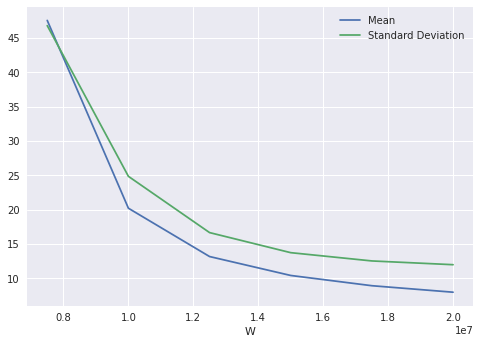
\includegraphics[width=\textwidth]{figures/e_coli-error_mean_stddev-K31-D6-T40}
        \caption{$d = 6$}\label{fig:ecoli-art-dbcm-errors-d6}
    \end{subfigure}%
    \begin{subfigure}{.5\textwidth}
        \centering
        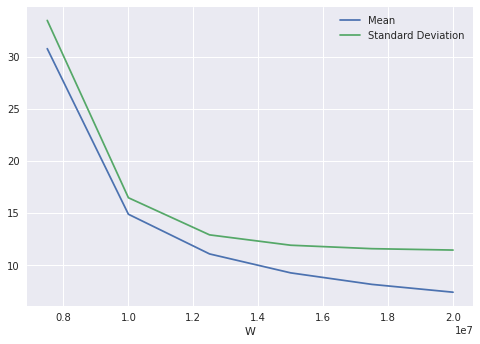
\includegraphics[width=\textwidth]{figures/e_coli-error_mean_stddev-K31-D8-T40}
        \caption{$d = 8$}\label{fig:ecoli-art-dbcm-errors-d8}
    \end{subfigure}
	\caption{\dBCM miscount mean and standard deviation as a function of $w$ for $d = 6$ and $d = 8$}\label{fig:ecoli-art-dbcm-errors}
\end{figure}

For $w \geq 10M$, we observe that both error mean and standard deviation are below $30$ regardless of $d$, such that we expect the majority, over $80\%$, of spurious \kmer{s} to have a count no greater than $60$, while real \kmer{s} are expected to have a count not much lower than $c=80$. This suggests that high- and low-frequency \kmer{s} are likely to still be discernible. To further determine how well the \dBCM can differentiate between these two categories, we select $w=10M$ and $d=6$, minimizing the memory used for the representation, and compare its count distribution for the \kmer{s} in the reads with the exact counts. This comparison can be observed in Figure~\ref{fig:ecoli-art-dbcm-counts}. Although the estimated counts distribution is shifted right due to overcount, we see two peaks, one between $2^3$ and $2^4$, and the other between $2^6$ and $2^7$, indicating the high- and low-frequency categories may still be discernible. An optimal threshold, however, is not as immediately clear as when we consider the exact count distribution.

\begin{figure}[htb]
    \centering
    \begin{subfigure}{.5\textwidth}
        \centering
        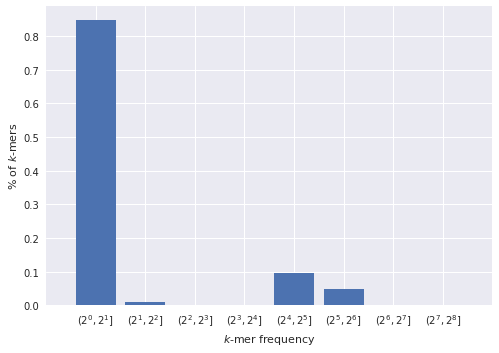
\includegraphics[width=\textwidth]{figures/e_coli-kmer_frequencies-exact-K31}
        \caption{Exact}\label{fig:ecoli-art-dbcm-counts-exact}
    \end{subfigure}%
    \begin{subfigure}{.5\textwidth}
        \centering
        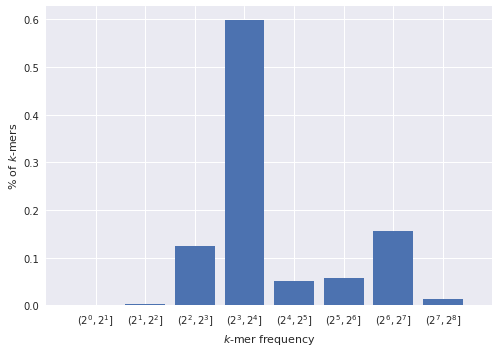
\includegraphics[width=\textwidth]{figures/e_coli-kmer_frequencies-estimated-K31-W10000000-D6}
        \caption{Estimated ($w = 12.5M, d = 6$)}\label{fig:ecoli-art-dbcm-counts-exact}
    \end{subfigure}
	\caption{\kmer count distribution}\label{fig:ecoli-art-dbcm-counts}
\end{figure}

To precisely determine how well we can categorize the \kmer{s} based on estimated count, we select a number of thresholds $t$ in the range $[1, 2c]$ and analyze the sensibility, i.e. percentage of true \kmer{s} idenfied as such, and false positive rate, i.e. percentage of false \kmer{s} erroneously identified as true, of using each one. The results are presented in Figure~\ref{fig:ecoli-art-dbcm-threshold-estimated}, where we can see that, without excluding any true \kmer{s} from the \dBG, we can filter out over $80\%$ of the spurious \kmer{s} from the reads by using $20 \leq t \leq 40$. However, comparing these results with the sensitivity and false positive rate if using the exact counts (Figure~\ref{fig:ecoli-art-dbcm-threshold-exact}), we can see that the number of false positives nearly doubles when keeping sensibility maximized. In the synthetic reads dataset used, this equates to nearly $9.7M$ spurious \kmer{s} being added to the \dBG, over $5M$ more than would be added using exact counts. In the following section we show that, despite this increase in number of spurious \kmer{s} represented in the \dBCM, only a fraction of them are reachable in traversal, such that this representation still succeeds in filtering out erroneous \kmer{s}.

\begin{figure}[htbp]
    \centering
    \begin{subfigure}{.5\textwidth}
        \centering
        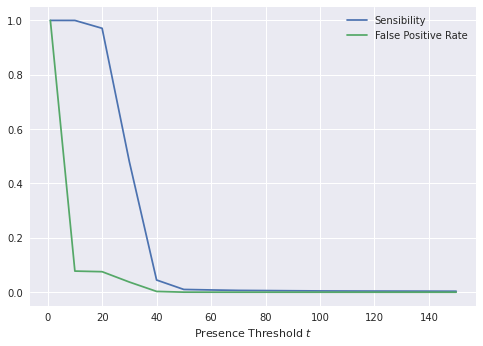
\includegraphics[width=\textwidth]{figures/e_coli-threshold_exploration-K31-exact}
        \caption{Exact counts}\label{fig:ecoli-art-dbcm-threshold-exact}
    \end{subfigure}%
    \begin{subfigure}{.5\textwidth}
        \centering
        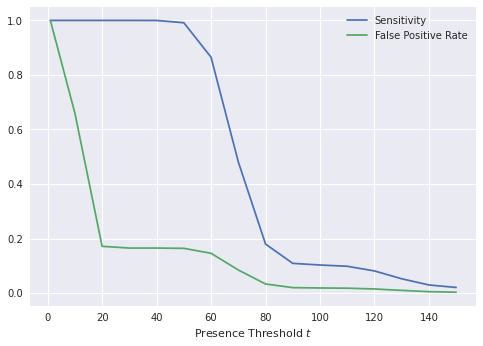
\includegraphics[width=\textwidth]{figures/e_coli-threshold_exploration-K31-W10000000-D6}
        \caption{Estimated by \dBCM ($W=10M, D=8$)}\label{fig:ecoli-art-dbcm-threshold-estimated}
    \end{subfigure}
    \caption{Sensibility and False Positive Rate of a \dBCM with $w = 12.5M$ and $d = 6$ as a function of the presence threshold $t$}\label{fig:ecoli-art-dbcm-threshold}
\end{figure}

\section{Further filtering through traversal}

AS discussed in Section~\ref{sec:pipeline}, we expect many of the spurious \kmer{s} inserted into the \dBG due to high count to be disconnected from the main component of the graph, composed of the real \kmer{s}. As such, the \kmer{s} categorized as high-frequency can further be filtered by traversing the graph from a starting set sampled from them

2. Navegação pelo dBCM
2.1. Navegação consegue melhorar FPR sem alterar sensibilidade?
Fig. FPR \& Sensibility X W (t = 40) [navegação]
2.3. Memória
2.3.1. Teórico
2.3.2. bits / kmer baseado nos \kmer{s} da navegação
2.4. Tempo
2.4.1. Construir, navegar

3. Navegação da dBHT
3.1. O quão próximo a dBHT consegue se manter da FPR do dBCM?
Fig. FPR \& Sensibility X alpha (W = 10M, D = 6 e t = 40) [navegação]
- $0.5 \leq alpha \leq 0.9$ (passo 0.05)
2.3. Memória
2.3.1. Teórico
2.3.2. bits / kmer baseado nos \kmer{s} da navegação
2.4. Tempo
2.4.1. Construir, navegar


\section{Theoretical Results}\asq{bad name}

\asq{This feels like it should be in methodology?}

$F => \|\readset\|_1$

Relationship between $c$, $t$, and $W$: a false positive occurs when $C.\mathit{query}(X).c - f(X) \geq t$, so we set $\epsilon F < t \rightarrow \epsilon < \frac{t}{F}$ in order to use Equation~\ref{eq:cm-prob} to establish a false positive rate. Because of the relationship $W = \frac{2}{\epsilon}$, we can put $W$ in terms of $t$: $W > \frac{2F}{t}$. Finally, we expect $F \approx c \times |\strname{S}|$, such that $W > \frac{2 \times c \times |\strname{S}|}{t}$.

Considering that there are approximately $2 \times |\strname{S}|$ distinct real \kmer{s} (including the reverse complements), we would use close to \asq{Close to because $W > \frac{2 \times c \times |\strname{S}|}{t}$, and here I'm considering $W =  \frac{2 \times c \times |\strname{S}|}{t}$} $\frac{c}{t} \times D \times 16$ bits per \kmer. It is clear, therefore, that using a higher value of $t$ is, theoretically, more space-efficient. Using $D = 8$ for an expected false positive rate of $\delta = 0.004$, and setting $t = \frac{c}{2}$, we expect to need 256 bits per \kmer. In this scenario, the \dBG for the \emph{E.~Coli} genome, with nearly 4.6Mb, would be represented in close to 147MB of memory. The human genome would need just over 200GB.

In practice we will show that this is an overestimate, as the sketch seems to perform better than expected.

\asq{Is it possible to create an expression for the false positive rate during traversal? It would depend on (a) the chance that a false \kmer is added to the starting set (so the chance that a false \kmer that appears at the beginning of a read is considered high-frequency) and (b) the chance that a real \kmer has a false edge pointing to a false \kmer}

\section{The \dBCM as a \dBG representation}

We started by evaluating how well the \dBCM performs the task of \kmer counting, comparing the distribution of frequencies, and observing the average error. However, because the goal of this data structure is to allow categorization of \kmer{s} as high- or low-frequency, more than obtaining exact \kmer counts, we take a special interest in evaluating how much the miscounts impact in differentiation between the two categories. To do this, we categorize the \kmer{s} according to a series of thresholds $t$, using both the exact frequency for each \kmer and the frequency estimated by the \dBCM. Let $H$ be the set of \kmer{s} categorized as high-frequency, and $K$ be the set of \kmer{s} found in the reference genome \strname{S} and its reverse complement \strname{\overline{S}}. We then generate $F_P = H \setminus K$, the set of spurious \kmer{s} that were considered to be high-frequency (false positives), and $F_N = K \setminus H$, the set of true \kmer{s} that were not considered to be high-frequency (false negatives). By analysing how the sizes of these sets varies as a function of $t$ we find the optimal threshold for differentiating the two categories.

Because the parameter $W$ has an important impact on the magnitude of the expected overcount, we analyze how they affect the error by comparing the mean and standard deviation for this metric across varying values of $W$.

We have used $D = 8$ as it gives a high degree of confidence in Equation~\ref{eq:cm-prob} (0.04\% chance of a miscount being greater than $\epsilon F$).

We selected an initial value of $W$ by estimating $t = 40$ as a good threshold value due to it being equidistant from the expected frequency of real \kmer{s} ($80$), and of spurious \kmer{s} ($1$). We then made $W = \frac{2F}{t} = 20M$. The distributions of the exact frequencies and those estimated by the resulting \dBCM sketch are presented side-by-side in Figure~\ref{fig:ecoli-art-frequencies}. We can see that the estimated frequencies are shifted right in relation to the exact frequencies, expected from the fact that the \dBCM will err by overcounting. However, we can see that the distribution remains clearly bimodal. Therefore, it is possible to choose a value $t$ that divides the \kmer{s} into the two categories.

\begin{figure}[htbp]
    \centering
    \begin{subfigure}{.5\textwidth}
        \centering
        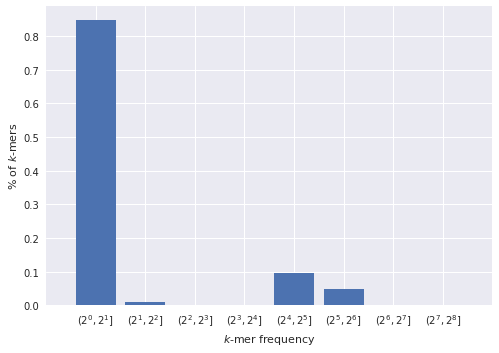
\includegraphics[width=\textwidth]{figures/e_coli-kmer_frequencies-exact-K31}
        \caption{Exact frequencies}\label{fig:ecoli-art-frequencies-exact}
    \end{subfigure}%
    \begin{subfigure}{.5\textwidth}
        \centering
        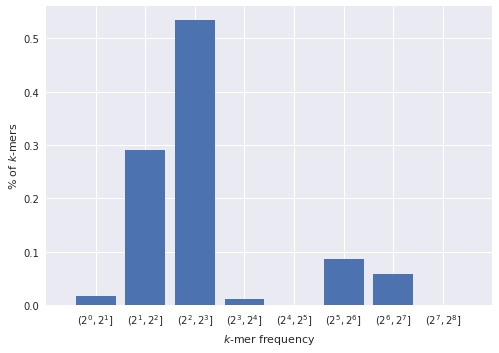
\includegraphics[width=\textwidth]{figures/e_coli-kmer_frequencies-estimated-K31-W20000000}
        \caption{Estimated frequencies}\label{fig:ecoli-art-frequencies-estimated}
    \end{subfigure}
	\caption{\kmer frequencies for \emph{E.~Coli} genome with $k=31$. \dBCM parameters: $(W=20M, D=8)$}\label{fig:ecoli-art-frequencies}
\end{figure}

Using the same count results, we selected values of $t \in \{1, 10, 20, \ldots, 160 (2 \times c)\}$ and compared the percentages of the true \kmer{s}, and of the spurious \kmer{s}, that were considered high-frequency. Figure~\ref{fig:ecoli-art-thresholds} presents the results when we use the exact counts for categorizing next to the results from using the estimated counts. Firstly, we can see that, when using either exact or estimated count, $t = 10$ is enough to filter out the majority of spurious \kmer{s}, further demonstrating that most of them appear a very low number of times in the reads. Moreover, we can see that the range of $t$ for which almost all real \kmer{s} are considered to be high-frequency is widened by using the estimated counts. This is to be expected, again, due to collisions and overcounting. Likewise, we see that $t$ must also be higher before we see the number of false \kmer{s} categorized as high-frequency diminish.

\begin{figure}[htbp]
    \centering
    \begin{subfigure}{.5\textwidth}
        \centering
        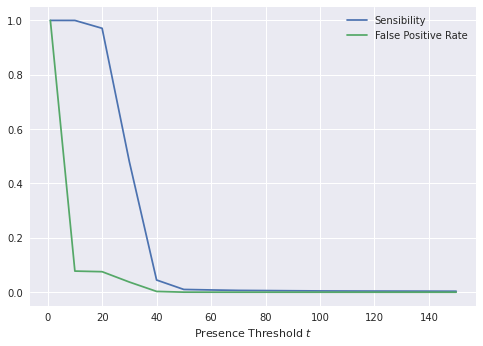
\includegraphics[width=\textwidth]{figures/e_coli-threshold_exploration-K31-exact}
        \caption{Exact counts}\label{fig:ecoli-art-threshold-exact}
    \end{subfigure}%
    \begin{subfigure}{.5\textwidth}
        \centering
        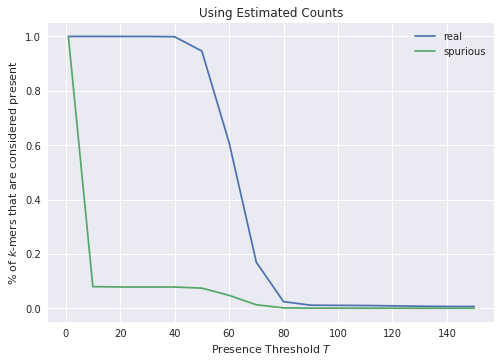
\includegraphics[width=\textwidth]{figures/e_coli-threshold_exploration-K31-W20000000-D8}
        \caption{Estimated by \dBCM ($W=20M, D=8$)}\label{fig:ecoli-art-frequencies-W20000000-D8}
    \end{subfigure}
    % \begin{subfigure}{.5\textwidth}
    %     \centering
    %     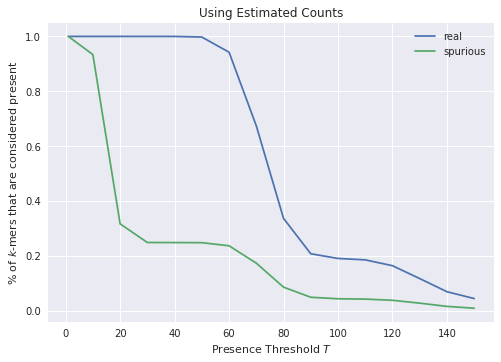
\includegraphics[width=\textwidth]{figures/e_coli-threshold_exploration-K31-W7500000-D8}
    %     \caption{Estimated by \dBCM ($W=7.5M, D=8$)}\label{fig:ecoli-art-frequencies-W7500000-D8}
    % \end{subfigure}
	\caption{Percentages of true and spurious \kmer{s} considered to be high-frequency according to different values of $t$ using (a) exact and (b) estimated counts (\dBCM parameters: $(W=20M, D=8)$).}\label{fig:ecoli-art-thresholds}
\end{figure}

We, then, iteratively lowered $W$ to evaluate how smaller sketches performed in \kmer counting, seeing how this affected the mean error, as well as the standard deviation. The results are seen in Figure~\ref{fig:ecoli-art-error}, where we plot the mean and standard deviation of the count errors as a function of $W \in \{5M, 7.5M, \ldots, 17.5M, 20M\}$. Because the spurious \kmer{s} appear a low number of times, analysing the mean error, as well as the standard deviation of the errors gives good insight into what kind of threshold would be needed to successfully categorize the \kmer{s} according to frequency, as we expect $50\%$ of \kmer{s} to have its count overestimated by the mean error or less, and over $80\%$ of \kmer{s} \toconsider{should} have a count that is overestimated by the mean plus one standard deviation. By analizing Figure~\ref{fig:ecoli-art-error}, we can see that there is little increase in the mean and standard deviation of the error from $W = 20M$ to $W = 10M$, with performance deteriorating much more quickly after that.

One interesting thing to note is that, with $W = 10M$, both the mean and the standard deviation of the error are below $20$, such that we expect over $80\%$ of the \kmer counts to not be overestimated by more than $40$. In fact, in Section~\ref{sec:traversal-results} we show that the \dBCM performs very well with $t = 40$ and $W = 10M$, half of the size suggested by Equation~\ref{eq:cm-prob}.

\begin{figure}[htbp]
    \centering
    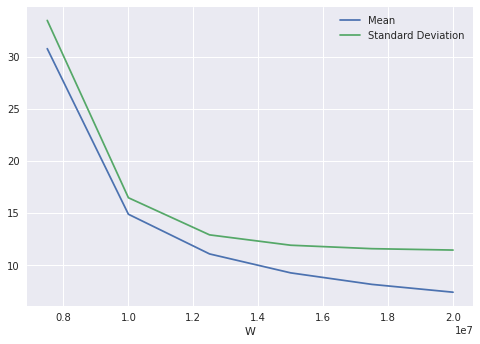
\includegraphics[width=0.9\textwidth]{figures/e_coli-error_mean_stddev-K31-D8-T40}
    \caption{Error mean and standard deviation as a function of $W$}\label{fig:ecoli-art-error}
\end{figure}

In Figure~\ref{fig:ecoli-art-W7500000} we replicate the results of the \dBCM from Figures~\ref{fig:ecoli-art-frequencies}~and~\ref{fig:ecoli-art-thresholds} for $W = 7.5M$, showing the other extreme of the range. \asq{Passar por aqui de novo, mas para mostrar o outro lado da range o correto seria mostrar $W = 5M$, e $W = 7M$ já apresenta um erro significativamente maior de forma que para representar o extremo ainda positivo, faria mais sentido usar $W = 10M$.}

\begin{figure}[htbp]
    \centering
    \caption{}\label{fig:ecoli-art-W7500000}
\end{figure}

\asq{Falar aqui sobre diminuir $D$?}

\asq{Teria sido possivel gerar algum valor que não seja o erro ou o desvio padrão que permita definir o quão bem aquele valor de $W$ consegue dividir os \kmer{s} nas duas categorias? Algo tipo: fazer a variação do $t$ e aí encontrar o $t$ que maximiza a diferença entre o percentual de \kmer{s} reais inclusos e o percentual de \kmer{s} espúrios, e aí usar essa diferença de percentual para determinar o quão bem aquele valor de $W$ consegue diferenciar as duas categorias?}

\subsection{Memory Usage}

We can express the number of bits per \kmer needed to represent the \dBG allowing for an expected false positive rate---the chance that a spurious \kmer will be considered high-frequency---$\delta$ in terms of the sequencing coverage $c$, and the presence threshold $t$ to be used. The total memory used is $16 \times W \times D$ bits, and we expect there to be $|\strname{S}|$ distinct \kmer{s} in the sequence. Because we add \kmer{s} both in forward and reverse complement direction, approximately $2 \times |\strname{S}|$ distinct \kmer{s} are represented in the \dBG. Benefiting from the fact that the majority of spurious \kmer{s} appear only once or twice in the reads, we can consider that they will only be considered high-frequency when they are miscounted by almost $t$. As such, we can express the false positive rate as $\prob[C.\mathit{query}(X) - f(X) > t]$, and use Equation~\ref{eq:cm-prob} to establish a relation between the size of the \dBCM, determined by $W$ and $D$, and the false positive rate in terms of $t$ by making $\epsilon F = t$. Because $F \approx c \times |\strname{S}|$, we can express $W = \frac{2 \times c \times |\strname{S}|}{t}$, while $D = \log(\frac{1}{\delta})$ remains the same. The total size of the \dBCM, then, is $16 \times \frac{2 \times c \times |\strname{S}|}{t} \times \log(\frac{1}{\delta})$ bits. Since we expect around $2 \times |\strname{S}|$ distinct \kmer{s} to be represented in the \dBG, we arrive at approximately $16 \times \lceil \frac{c}{t} \rceil \times \lceil \log(\frac{1}{\delta}) \rceil$ bits per \kmer. Choosing $t = \frac{c}{2}$ and a desired false positive rate of $1\%$, we expect the \dBCM to need $147$ bits per \kmer.

\asq{Um problema sério dessa sessão é que, na prática, a taxa de falsos positivos vai ser mais alta do que o valor definido. Isso acontece porque existe uma quantidade de \kmer{s} espúrios que tem um contagem maior do que 1 ou 2, de forma que a garantia de $C.\mathit{query}(X) - f(X) \leq t$ é uma garantia fraca. Para eliminar esses \kmer{s} seria necessário definir o erro máximo aceito como um valor menor do que o threshold de presença (i.e. $C.\mathit{query}(X) - f(X) \leq t - \beta$). Não sei se tem alguma forma de definir esse valor de forma sistemática (e.g. qual é o menor threshold para o qual, baseado na contagem real, esperamos cortar $90\%$ dos \kmer{s} espúrios?) Talvez seja possível chegar a tal expressão baseado na probabilidade do erro, e a probabilidade de dois erros distintos gerarem o mesmo \kmer, mas acredito que seria uma expressão complexa.}

\section{Traversal of the \dBCM}
\label{sec:results-dbcm-traversal}

The previous results suggest that the \dBCM is possibly an apt representation of the \dBG as an MDS, with its expected false positive rate for $W = 20M$ being below $20\%$, as can be extrapolated from the percentage of spurious \kmer{s} categorized as high-frequency. Although not ideal, it is likely not high enough to \toconsider{disrupt} usage of the graph \cite{Pell2012}. However, we expect the addition of outedges to improve on the navigability of the graph, resulting in an even lower false positive rate in practice, as the graph is traversed.

To test this, we traversed the \dBCM starting from a set of known member nodes selected during construction of the graph by picking the first \kmer of each read if its count already surpassed $t$. During traversal, we register all the \kmer{s} that are queried from the \dBCM (which we call $Q$), as well as the query result. With this data, we evaluate how many \kmer{s} are queried during traversal, and how many of those are actually found to be in the graph (we refer to the set of \kmer{s} found during traversal as $V$). We can, then, define the set of false positives $F_P = V \setminus K$ and the set of false negatives as $F_N = K \setminus V$. We establish the false positive rate as $f_p = \frac{|F_P|}{|V|}$ and the false negative rate as $f_n = \frac{|F_N|}{|K|}$.

\asq{Aqui vale colocar alguns resultados e gráficos para uma instância específica (talvez $W = 20M$ de novo), como, por exemplo, a distribuição do número de arestas em cada nó visitado. Isso deve permitir entender o porque de a taxa de falsos positivos crescer tão rapidamente aparentemente de repente.}

Figure~\ref{fig:ecoli-art-traversal-W-queriedfound} presents the number of \kmer{s} queried and found during traversal for different \dBCM with different parameters $W$ \asq{Importante notar que são usados os mesmos valores de $W$ que antes, exceto por $W = 5M$, que foi excluído porque, devido a alta taxa de falsos positivos, o programa estoura a memória e é interrompido sem gerar resultados}. Figure~\ref{fig:ecoli-art-traversal-W-fpfn} shows the false positive and false negative rates as a function of $W$.

\begin{figure}[htbp]
	\centering
    \begin{subfigure}{.5\textwidth}
        \centering
        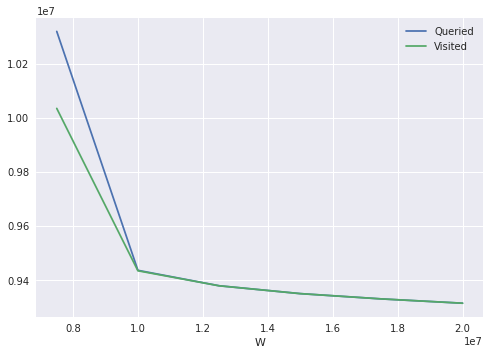
\includegraphics[width=\textwidth]{figures/e_coli-dbcm-queried_and_found-K31-D8-T40}
        \caption{Queried \& Found}\label{fig:ecoli-art-traversal-W-queriedfound}
    \end{subfigure}%
    \begin{subfigure}{.5\textwidth}
        \centering
        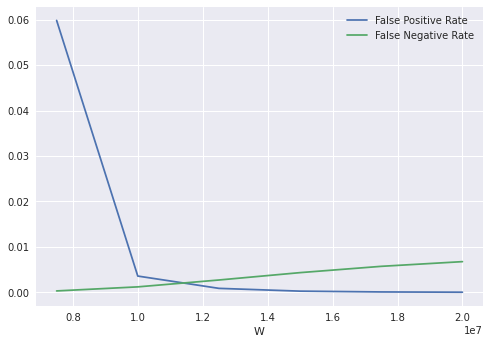
\includegraphics[width=\textwidth]{figures/e_coli-dbcm-false_positive_and_negative_rates-K31-D8-T40}
        \caption{False Positives}\label{fig:ecoli-art-traversal-W-fpfn}
    \end{subfigure}
	\caption{Number of (a) \kmer{s} queried and found during traversal and (b) false positives}\label{fig:ecoli-art-traversal-W}
\end{figure}

\section{Construction of the \dBHT from the \dBCM}

\asq{Trazer informações aqui sobre o tempo necessário para a construção da nova estrutura}

\section{Traversal of the \dBHT}

\asq{Trazer os mesmos gráficos da Seção~\ref{sec:results-dbcm-traversal} sendo que para a \dBHT. Falar sobre como ela tem uma taxa de falsos positivos maior do que a \dBCM, apesar de apenas os nós visitados na \dBCM serem adicionados na \dBHT e as arestas ainda passarem por uma limpeza (arestaas que não apontam para um nó real no \dBCM não são adicionadas na \dBHT). Isso provavelmente acontece porque usar 8 hashes distintos previne mais colisões do que apenas um hash e um fingerprint.}